\documentclass {report}
\usepackage[utf8]{inputenc}

\usepackage{polyglossia}
\usepackage{graphicx}
\usepackage{fancyvrb}
\usepackage{circuitikz}
\usepackage{pgfplots}
\usepackage{geometry}
\usepackage{graphics}
\usepackage{hyperref}
 \geometry{
 a4paper,
 total={170mm,257mm},
 left=10mm,
 top=20mm,
 }

\title{Elektrisku shēmu modelēšana}
\author{Diāna Dupļevska}
\date{2019. 13. marts}

\begin{document}

\maketitle
\chapter{Teorētiskā daļa}
\section{Ķēdes aprēķins}
\begin{center}
\small\addtolength{\tabcolsep}{10pt}
\subsection{Ķēde}
\begin{circuitikz}[scale=1, every node/.style={transform shape}]
\draw
(0,0) to [short, *-] (6,0)
  to [V, l_=$\mathrm{j}{\omega}_m \underline{\psi}^s_R$] (6,2) 
  to [R, l_=$R_R$] (6,4) 
  to [short, i_=$\underline{i}^s_R$] (5,4) 
  (0,0) to [open, v^>=$\underline{u}^s_s$] (0,4) 
  to [short, *- ,i=$\underline{i}^s_s$] (1,4) 
  to [R, l=$R_s$] (3,4)
  to [L, l=$L_{\sigma}$] (5,4) 
  to [short, i_=$\underline{i}^s_M$] (5,3) 
  to [L, l_=$L_M$] (5,0);
\end{circuitikz}
\end{center}
\begin{center}
\small\addtolength{\tabcolsep}{10pt}
\begin{center}
\subsection{Tabula ar datiem}
\caption{Tas ir tabulas virsraksts}\\
\label{i:example}
\begin{tabular}{|c|c|}
\hline \multicolumn{2}{|c|}{Tabula:} \\
\hline
R1 & 7Ω\\
\hline
R2 & 9Ω\\
\hline
V1 & 36.8V\\
\hline
$U_{R1}$ & 16.1V\\
\hline
$U_{R2}$ & 20.7V\\
\hline
\end{tabular}
\end{center}
\section{Oma likums}
\Label{sec:Oma}
\textbf{Spriegumu U{R1} es aprekināju izmantojot Oma likumus}\cite{gramata1}
\subsection{Grafiks}
\begin{tikzpicture}
\begin{axis}[]
\addplot [black, very thick]{x*x};
\end{axis}
\end{tikzpicture}
\end{center}
\chapter{Praktiskā daļa}
\section{Darbs ar gEDA programmām}
\subsection{Darbs ar gschem}

\begin{figure}
\rotatebox{-90}{\includegraphics[width=15cm,height=15cm,keepaspectratio]{01.ps}}\\
\caption{1.attēls}
\label{i:example}
\end{figure}

\subsection{Darbs ar gnetlist}
\VerbatimInput{01.net} \\

\begin{figure}
    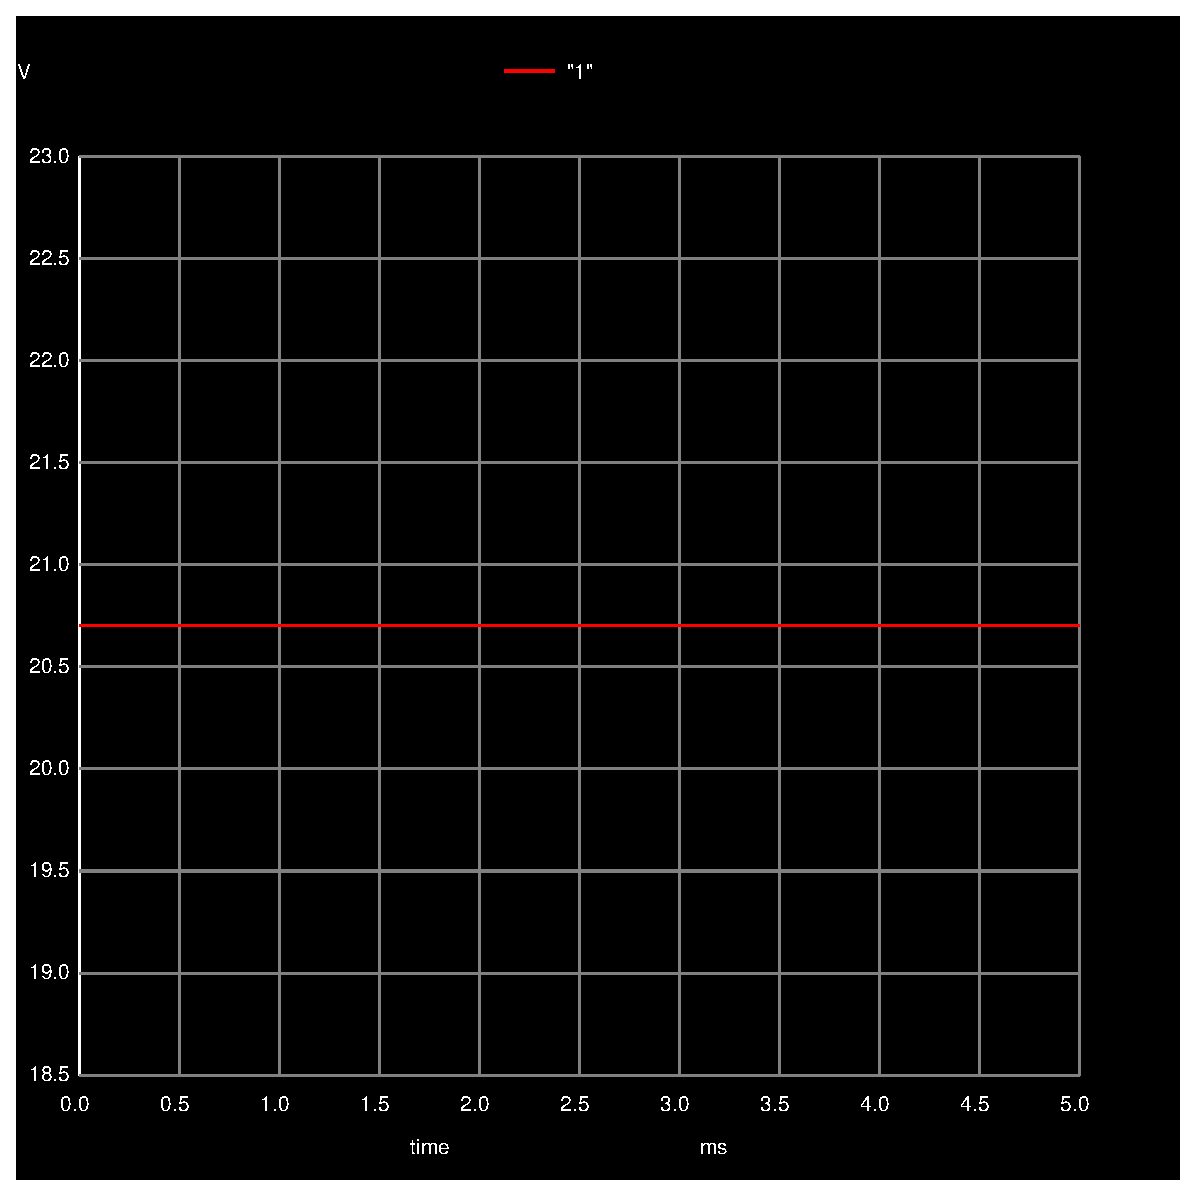
\includegraphics[width=12cm,height=12cm,keepaspectratio]{011.ps}  \\
\caption{2.attēls}
\label{i:example}
\end{figure}
\begin{figure}
    \includegraphics[width=12cm,height=12cm,keepaspectratio]{022.ps}  \\
  \caption{3.attēls}
\label{i:example}
\end{figure}
  
    
\section{Darbs ar QUCS programmām}
\VerbatimInput{02.sch}
\textbf{Līdzstrāvas simulācijas grafiks:}

\begin{figure}
\rotatebox{-90}{\includegraphics[keepaspectratio]{result2.ps}}\\
\caption{4.attēls}
\label{i:example}
\end{figure}

\textbf{Sweep simulācijas līdzstrāvas grafiks un tabula:}

\begin{figure}
\rotatebox{-90}{\includegraphics[keepaspectratio]{result.ps}}\\
\caption{5.attēls}
\label{i:example}
\end{figure}
\begin{thebibliography}{9}
\bibitem{gramata1}
\hyperref[sec:Oma]{Word of text}
Strauts, A. Elektrotehnikas teorētiskie pamati: lekciju konspekts. Rīga: RTU, 2007. {\label{mans_id}}
\bibitem{gramata2}
Boctor, S.A. Circuit Analysis. New Jersey: Prentice Hall, 1987.
\end{thebibliography}
\end{document}